\label{chap.3}
\section {Chapter Introduction}
This chapter will introduce the proposed methodology on how to approach the challenge of early plant disease detection and identification by implementing AI and DL approaches. It references the study based on literature and points out how the proposed program meets the need for contemporary research in eliminating the deficits and barriers present. Finally, the chapter highlights the novelty and uniqueness of the proposed framework to be not only resource-friendly but also user-friendly to the nonscientific individual.
\section{Proposed Work}
% Provide an overview of the proposed work, connecting it to the research gaps identified in the Literature Study chapter.
% Briefly restate the problem.
% Highlight how your proposed work addresses the gaps or challenges.
% Emphasize the novelty or uniqueness of your approach.

Modern agricultural methods face severe challenges that arise from plant diseases, leading to a decrease in crop production and monetary loss. Early diagnosis of plant diseases is thus very critical to overcome such impacts. However, available methods are resource-intensive, require expert intervention, and are not scalable. The purpose of our proposed study is to develop an artificial intelligence-based system that helps detect plant diseases early, but with low resource intensity and infrastructure requirements. The focus should be on developing a solution that is cost-effective, user-friendly, and easily accessible to farmers and agriculturalists, especially those who are in remote or resource-limited areas.

\

Through an extensive review of existing literature and current methodologies in plant disease detection systems, several critical gaps and limitations have been identified that significantly impact the practical implementation and accessibility of these solutions. A primary concern is the heavy reliance on sophisticated and expensive equipment, including high-resolution imaging systems, specialized sensors, and advanced computational hardware. This dependence on costly infrastructure creates a substantial barrier for small-scale farmers and agricultural communities with limited resources, effectively excluding a significant portion of the target user base from accessing these technological advancements. Furthermore, the existing solutions demonstrate a notable limitation in dataset diversity, with many systems being developed and trained on narrow, crop-specific datasets. This specialization, while potentially beneficial for specific applications, severely restricts the systems' generalizability and adaptability across different agricultural contexts and varied crop types. The challenge of real-time analysis presents another significant hurdle, as numerous existing systems operate primarily through offline processing mechanisms, introducing considerable delays between disease detection and implementation of remedial measures. This delay can be critical in agricultural scenarios where rapid response is essential for disease containment and crop preservation. The complexity in deployment represents another substantial barrier, with many current solutions requiring extensive technical expertise and sophisticated computational resources for successful implementation. This technical complexity makes these systems particularly impractical for deployment in rural and remote agricultural areas, where technical support and infrastructure may be limited. Additionally, scalability emerges as a crucial concern, as few existing approaches have successfully developed frameworks that can be readily adapted and scaled across different crop varieties and disease types while maintaining accuracy and efficiency. The integration challenges with contemporary mobile and web-based platforms further compound these limitations, as many systems lack user-friendly interfaces and accessible deployment options that would make them practical tools for farmers and agricultural workers. These technological and accessibility barriers collectively highlight the pressing need for more inclusive, scalable, and practically implementable solutions in plant disease detection systems.

\

The research initiative seeks to fill critical gaps in the detection of agricultural diseases through the introduction of a our application that exploits the power of artificial intelligence and machine learning technologies. This detailed approach begins with a focused study of the leaf curl virus, one of the most damaging plant pathogens, with a massive impact on crop productivity worldwide. This concentrated approach makes it easier to lay a strong foundation that can then be expanded to encompass a more diverse range of plant diseases impacting different species. The implementation of this method relies heavily on sophisticated convolutional neural network architectures that are designed specifically to operate efficiently on resource-constrained devices, like smartphones. The framework effectively realizes advanced feature extraction while preserving computational efficiency by applying transfer learning methodologies utilizing well-established architectures such as MobileNetV2 and EfficientNet. A fundamental aspect of the initiative consists of the careful assembly of a comprehensive dataset, which is enhanced by sophisticated data augmentation strategies that improve the model's robustness against real-world fluctuations in imaging conditions.

\

The proposed research is unique in being innovative and comprehensive in addressing the democratization of agricultural disease detection technology, especially looking at its implementation in resource-limited rural settings. The newness of the framework actually comes from its carefully planned methodology: starting with specialization in the leaf curl virus detection as a proof of concept and then expanding. Unlike traditional solutions that are mainly based on high-end server infrastructure, this approach focuses on efficiency and accessibility through optimized lightweight architectures designed for mobile devices without compromising the accuracy of detection. One of the most outstanding features of the framework is the sophisticated integration of traditional machine learning methodologies with cutting-edge deep learning architectures, making it a hybrid system that adapts dynamically to varying conditions and requirements. The solution's robustness is enhanced by an extremely curated dataset encompassing a multiplicity of crop varieties and disease conditions, thereby highly enhancing the generalizability of the system across different agricultural contexts. The framework emphasizes user accessibility through thoughtfully designed interfaces that provide clear actionable insights, making advanced technology accessible to users with varied technical expertise. Perhaps most significantly, the offline functionality allows reliable operation in areas where only limited internet connectivity exists, covering a critical gap left so far by existing solutions.

\

Implementation of the strategy follows a systematized progression starting off with comprehensive data collection as well as preprocessing to assure a robust foundation for models to be developed. This is the gathering of diverse samples of pictures of healthy and diseased plants from various sources to broaden representation across the conditions being represented. The model development phase of this process would focus more on training and optimizing these lightweight and deep learning architectures, with an emphasis more on maintaining performance but now at reduced computational costs. A critical aspect of the implementation involves rigorous optimization procedures to minimize model size and enhance inference speed, ensuring practical usability on mobile devices. The development of intuitive user interfaces, both mobile and web-based, forms a crucial component of the implementation plan, facilitating seamless interaction between users and the technology. The framework is tested and validated on the basis of comprehensive performance metrics, such as accuracy, precision, recall, and F1-score, to ensure its reliability across various operational conditions. The final phase includes careful deployment across mobile platforms and thorough field testing with actual farmers to validate real-world effectiveness and gather valuable user feedback for continuous improvement.

\subsection{ Objectives of the Proposed Work}
%  Clearly articulate the specific objectives of the proposed research or system.

% Define measurable goals.
% Include both primary and secondary objectives.

This research initiative is fundamentally driven by the hypothesis that early plant disease detection and intervention can be democratized through artificial intelligence solutions optimized for commonly available consumer hardware. The core premise suggests that by leveraging advanced machine learning techniques while prioritizing accessibility, it is possible to develop a practical system that enables timely disease identification and provides actionable intervention strategies, ultimately empowering farmers regardless of their technological infrastructure. The research aims to establish comprehensive documentation of various AI and ML methodologies' effectiveness in plant disease detection, with a particular focus on edge computing capabilities through mobile applications. This practical implementation goal is complemented by rigorous academic objectives, including the development of lightweight yet robust AI architectures capable of real-time disease detection while maintaining high accuracy levels suitable for field deployment. The project emphasizes creating an accessible system that significantly reduces reliance on expensive specialized equipment or consistent internet connectivity, thereby addressing a critical barrier to technology adoption in agricultural communities. Through intuitive user interface design and optimization for consumer-grade hardware, the research seeks to bridge the gap between sophisticated AI capabilities and practical agricultural needs. The anticipated impact extends beyond technological advancement, targeting tangible improvements in crop yield through early disease detection and intervention, ultimately contributing to agricultural sustainability and economic efficiency. This comprehensive approach represents a synthesis of technical innovation and practical utility, aiming to deliver a solution that is both scientifically rigorous and immediately applicable in real-world farming contexts.

The research endeavors to advance agricultural disease management through a comprehensive set of primary and secondary objectives that combine technical sophistication with practical utility. At its core, the project aims to develop a high-performance AI-based solution achieving a minimum 90\% accuracy rate in plant disease detection, while maintaining real-time processing capabilities with sub-second response times per image analysis. This technical precision is balanced with accessibility considerations, as the system is specifically engineered to operate efficiently on resource-constrained hardware platforms such as mobile devices and Raspberry Pi units. The initial focus centers on achieving exceptional accuracy in leaf curl virus detection, with a planned expansion to encompass at least five additional plant diseases, demonstrating the solution's scalability and versatility. A critical technical objective involves implementing robust offline functionality, ensuring the system's utility in regions with limited internet connectivity, while simultaneously developing sophisticated time-series prediction models to analyze and forecast disease progression patterns, enabling proactive intervention strategies.

Beyond these primary technical goals, the project encompasses several crucial secondary objectives aimed at maximizing real-world impact and usability. These include the development of an intuitive user interface designed specifically for non-technical users, incorporating clear visual feedback and actionable insights. The system will integrate comprehensive disease management recommendations, providing users with specific preventive measures and treatment options based on detection results. To ensure robust performance across diverse agricultural contexts, the framework will undergo rigorous evaluation using multiple datasets, complemented by extensive field trials and systematic user feedback collection. This practical validation phase will inform continuous refinement of both accuracy and usability aspects. Furthermore, the project emphasizes thorough documentation and architectural optimization to facilitate future expansion, establishing a foundation for incorporating additional plant species and diseases as the system evolves. This comprehensive approach ensures that the solution not only meets immediate agricultural needs but also provides a sustainable platform for ongoing development and adaptation to emerging challenges in plant disease management.

\section{ Methodology}
%  Describe the methods, techniques, and tools to be employed.
% Provide a detailed explanation of your approach.
% Include algorithms, frameworks, models, and workflows.
% Use diagrams to explain the methodology clearly.



\subsection{Overview of the Approach:} 
% A summary of your method.
The prime goal of this research endeavors to revolutionize plant disease detection by focusing on developing an integrated solution that harnesses the power of AI into robust as well as accessible health knowledge. The system thereby aims at merging computer vision techniques with natural language processing capabilities to evolve into a comprehensive diagnostic tool that can be transformed from mere disease identification into an interactive, context-aware treatment recommendation. 

\

In conclusion, solution architecture was carefully structured into various phased processes that are seamlessly linked for maximum effectiveness and reliability. The first part concerns complex data preprocessing aimed to obtain high-quality inputs consistently independent of the imaging environment conditions. The second was heavily modeled training using convolutional neural networks (CNN) and vision transformers, designed for high-precision detection of diseases. The integration of vision transformers is one great advancement, as architectures proved to be superior to all others in capturing long-range dependencies and contextual information inside images.

\

Particularly innovative within this system is its use of a Retrieval-Augmented Generation, or RAG, pipeline that improves the ability of the chatbot to produce the right answers at the right times. This enables it to dynamically access and draw on a curated knowledge base while ensuring that recommendations are not only scientifically sound but also practically applicable. The chatbot component transforms complex diagnostic information into accessible, conversational guidance, making the technology more approachable for users with varying levels of technical expertise.

\

This validation and real-world testing in the workflow indicates a commitment to the practical applicability of such a system, ensuring its reliability under various agricultural conditions. This all-inclusive approach creates a bridge between highly sophisticated AI technologies and real practical needs in agriculture and can transform the way farmers and agricultural professionals approach the management of plant diseases.

\subsection{Dataset Selection:}
% Describe the datasets (real-world, synthetic, or benchmarks) used for evaluation.

The dataset for training the model is a careful combination of the following datasets and the images directly collected with the courtesy of Amrita Coimbatore.

\

Plant-Doc dataset: https://github.com/pratikkayal/PlantDoc-Dataset 

PlantVillage dataset: https://www.kaggle.com/datasets/emmarex/plantdisease

iBean dataset: https://github.com/AI-Lab-Makerere/ibean

Citrus leaves dataset : https://www.tensorflow.org/datasets/catalog/citrus\_leaves

Rice Leaf Disease dataset: https://www.kaggle.com/datasets/vbookshelf/rice-leaf-diseases

\

The dataset finally prepared has approximately 21000 images spanning across 17 classes of plants.

\

 \textbf{Note:} The number of images in some classes in the dataset prepared is significantly lower compared to the other classes. This imbalance is a result of the compilation of multiple data sources to prepare a master dataset with maximum available data. This makes the problem a long-tail classification problem which can be solved through some preprocessing methods and training methods


 \begin{figure}[h!]
    \centering
    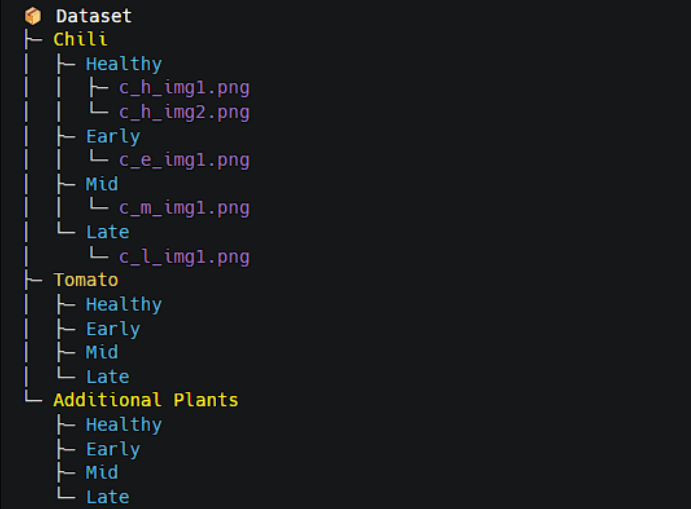
\includegraphics[scale=0.5]{ds.png}
    \caption{Structure of the dataset}
    \label{fig:dataset_structure}
\end{figure}


\

The dataset is structured to easily incorporate new data, with training data organized by prediction classes. One key challenge is the class imbalance in the dataset, where some categories have significantly fewer samples than others. This imbalance comes from combining different source datasets and creates what's known as a long-tail classification problem, requiring special handling during preprocessing and training.

The preprocessing pipeline is optimized for Vision Transformer architecture. Since the source data varies in image size, format, and capture conditions, we've established a standard preprocessing workflow. All images are rescaled to 224 x 224 resolution before going through the ViT preprocessor for patch-wise processing. This preprocessing adapts to different model architectures, and we plan to add disease progression data in future updates.

For language modeling, we use the Llama 3.2 2b model with a Retrieval-Augmented Generation (RAG) pipeline, avoiding the need for full model fine-tuning. We maintain a curated knowledge base that's embedded in a vector database for contextual information retrieval. To improve system efficiency, common questions about plant conditions are provided during prediction to reduce the language model's workload.

Training happens in two phases. First, we start with pre-trained Vision Transformer weights and update the entire network for plant disease detection, using best weight restoration to prevent overfitting and validation on separate test data. The system saves checkpoints regularly to handle any training interruptions. The second phase addresses the class imbalance through balanced retraining with frozen backbone weights. When adding new classes, both phases are repeated using the previous weights as starting points.

This approach creates a solid foundation for plant disease detection while staying flexible for future improvements. It effectively handles common agricultural image classification challenges while providing room for system growth.




\subsection{Algorithm/Model Design:}
% Explain the model architecture, algorithmic steps, or computational processes.
\begin{itemize}

\item \textbf{Vision Model:}
\begin{itemize}
\item \textbf{Pretrained Vision Transformer (ViT):} Extracts hierarchical visual features for disease classification.
\item \textbf{Custom CNN Layers:} Fine-tuned layers to improve feature extraction.
\item \textbf{Transfer Learning:} Utilizes pre-trained weights to accelerate training and optimize accuracy.
\end{itemize}

\item \textbf{Language Model:}
\begin{itemize}
\item \textbf{LLaMA 3.2 LLM:} Used for interactive chatbot responses with domain-specific customization.
\item \textbf{RAG Pipeline:} Enhances text generation by integrating document retrieval for contextual answers.
\end{itemize}

\end{itemize}

The classification framework uses a dual approach that combines visual and language processing components. The visual analysis uses Vision Transformer architecture to analyze images, identifying key signs of plant diseases through changes in leaf color, texture patterns, and structural damage.

The system performs image segmentation to separate diseased areas from healthy plant tissue, which helps the model focus on relevant features while reducing background interference. The transformer then processes these segments through multiple attention layers to understand both detailed and overall context needed for accurate disease identification.

The language processing component uses semantic similarity search through a vector database of agricultural knowledge. This database converts information about diseases, characteristics, and treatments into vector embeddings that preserve relationships between concepts, allowing quick retrieval of relevant information when a disease is identified.

By integrating these visual and text processing systems, the framework provides both accurate disease diagnosis and practical management recommendations for farmers.

\subsection{Tools and Technologies:} 
% Mention the programming languages, libraries, or software used.System Architecture/Design (Optional, for implementation-based projects)
% Provide a high-level view of the system's components and interactions.
% Include block diagrams or flowcharts to illustrate the design.
% Describe individual components and their roles.

\begin{itemize}

\item \textbf{Programming Languages:}
\begin{itemize}
\item Python, Node.js
\end{itemize}

\item \textbf{Libraries and Frameworks:}
\begin{itemize}
\item TensorFlow, PyTorch, OpenCV, Scikit-learn, Keras
\end{itemize}

\item \textbf{Vector Database:}
\begin{itemize}
\item ChromaDB for storing embeddings
\end{itemize}

\item \textbf{Deployment Tools:}
\begin{itemize}
\item Docker for containerization, Hugging Face for cloud hosting
\end{itemize}

\item \textbf{Mobile Development:}
\begin{itemize}
\item Flutter for cross-platform app development
\end{itemize}

\item \textbf{Version Control:}
\begin{itemize}
\item GitHub repositories for modular development
\end{itemize}

\end{itemize}

The current stage of this project is primarily focused on early development and prototyping, necessitating a cost-efficient and resource-conscious approach to implementation. Given the inherent limitations of free cloud services, the architecture emphasizes a decentralized design to ensure scalability and flexibility. At its core, the system is structured as a network of microservices, each of which is tasked with a specific, well-defined responsibility. This modular approach not only simplifies development and maintenance but also facilitates seamless integration and future scalability. Notably, the system does not mandate users to authenticate or provide any personal information, ensuring privacy and accessibility. Instead, each instance of a prediction operates within its own self-contained context, with all relevant data and results stored locally on the user’s device.

Currently, the prediction and language processing systems are hosted online, offering promising capabilities in addressing the identified problem domain. However, there remains considerable scope for improving their performance and expanding their utility. At this stage, the language model relies on a predefined set of static answers tailored to a limited range of frequently asked questions, specifically focusing on diagnosing a single type of plant disease. Ongoing development efforts aim to transition from this rudimentary setup to a more comprehensive, full-text processing system. The end goal is to deploy this enhanced model across multiple low-resource servers, leveraging freely available hosting solutions to ensure widespread accessibility without incurring significant costs.


\begin{figure}[h!]
    \centering
    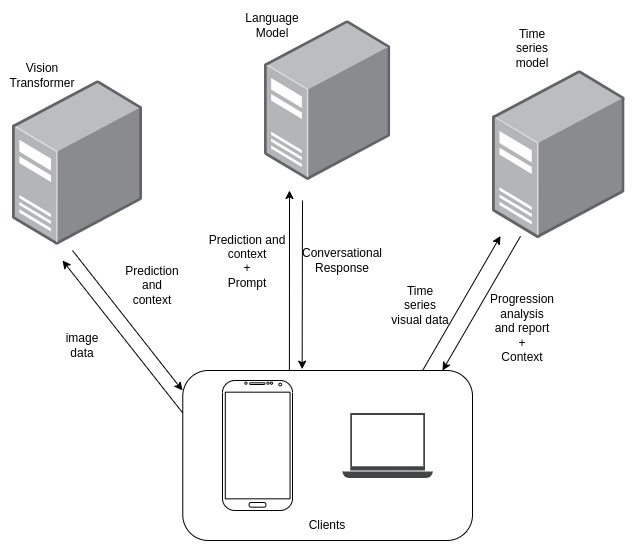
\includegraphics[scale=0.5]{architecture.jpg}
    \caption{Client-Server Architecture}
    \label{fig:client_server_arch}
\end{figure}


\begin{figure}[h!]
    \centering
    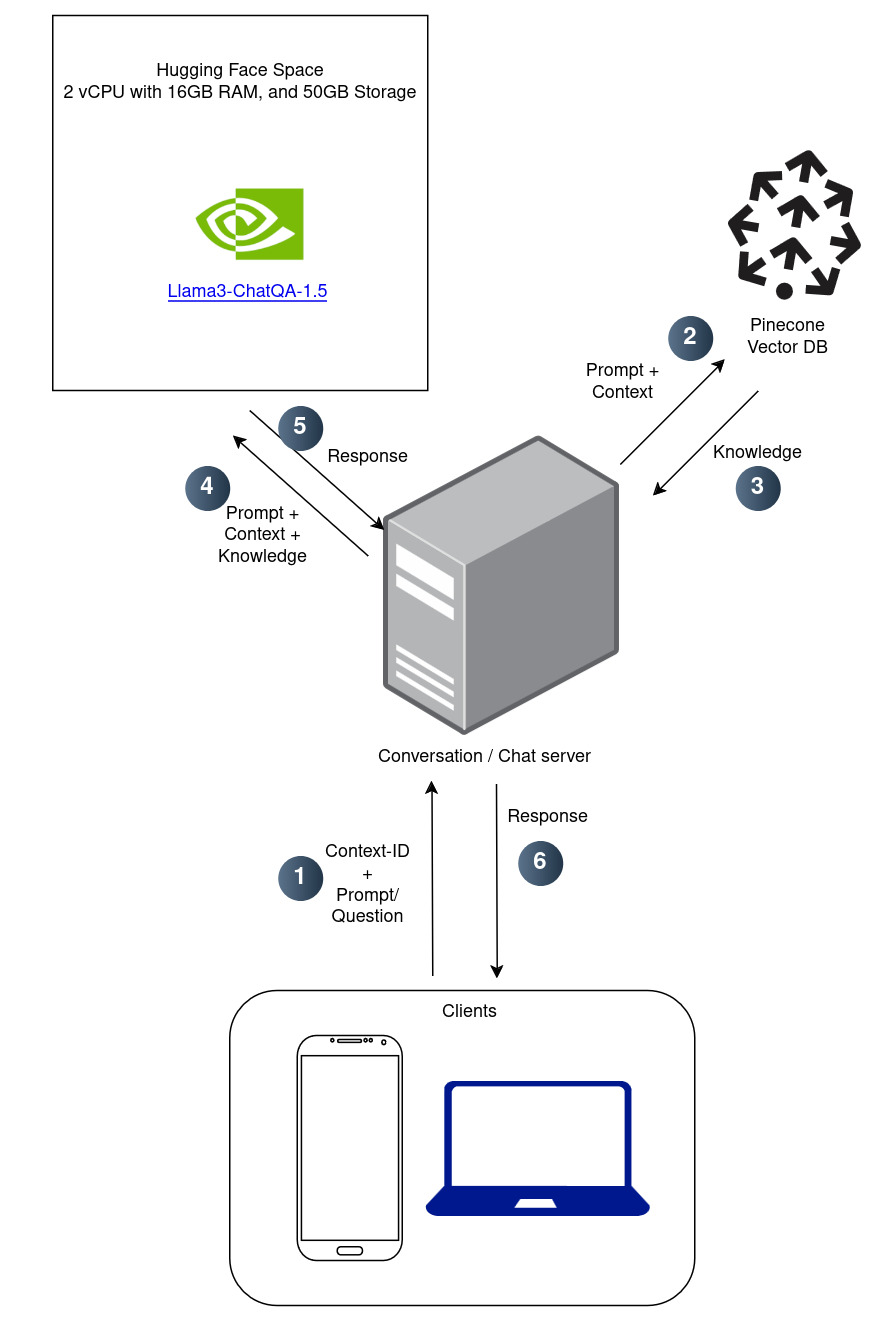
\includegraphics[scale=0.5]{images/chatbot_arch.jpg}
    \caption{Chatbot Architecture}
    \label{fig:chatbot_arch}
\end{figure}


\subsection{Algorithm or Model Description}



% Explain the model architecture, algorithmic steps, or computational processes.

% Also give explanation of how these algorithms are used in solving the problems. The prerequisites, if any, need to be explained.
% Any equations to clarify the algorithms, if necessary, may also be given.\\

The plant disease classification system uses a multi-stage pipeline focused on accuracy, dynamism, and practical usability. It starts with image preprocessing, where images are standardized through resizing, normalization, and augmentation. This ensures the model can handle different lighting conditions, angles, and image resolutions effectively.

For feature extraction, the system uses a Vision Transformer (ViT) that divides images into smaller patches. These patches are converted into embeddings that maintain spatial and structural information, capturing important details for disease identification. The ViT's self-attention mechanisms allow it to understand both local details and overall patterns in images better than traditional CNNs.

Training involves fine-tuning a pre-trained ViT model specifically for plant disease classification. To handle uneven distribution of disease classes in agricultural datasets, the system uses weighted loss functions - Binary Cross-Entropy for two-class problems and Categorical Cross-Entropy for multiple classes. These functions are optimized to improve prediction accuracy.

The validation process evaluates performance using multiple metrics: accuracy for overall correctness, precision for reliability of positive predictions, recall for ability to find positive cases, and F1-score for balanced performance measurement. This helps identify and address any training issues.

After validation confirms good performance, the model is deployed to classify new images. The deployment system is optimized to work efficiently, even on basic devices, providing disease predictions with confidence scores.

The system includes a RAG-powered chatbot that helps users interact with the results. This chatbot combines classification results with stored information to provide specific guidance about disease management, treatment options, and prevention strategies, making the system more practical and user-friendly.

 

From a mathematical standpoint, the model’s optimization process relies on minimizing the specified loss functions. Binary Cross-Entropy, defined as:  

\[
L = -\frac{1}{N} \sum_{i=1}^{N} \left[ y_i \log(p_i) + (1 - y_i) \log(1 - p_i) \right]
\]  

is used for binary classification, while Categorical Cross-Entropy, expressed as:  

\[
L = -\sum_{i=1}^{N} \sum_{j=1}^{C} y_{ij} \log(p_{ij})
\]  

is employed for multi-class scenarios. Here, \( y_i \) and \( p_i \) represent the true and predicted labels, respectively.  

The final layer of the model utilizes the Softmax activation function, given by:  

\[
\sigma(z_i) = \frac{e^{z_i}}{\sum_{j=1}^{C} e^{z_j}}
\]  

where \( z_i \) represents the logits for class \( i \), and \( C \) denotes the number of classes. This function transforms raw logits into probability distributions, enabling the system to determine the most likely disease category.  

The main overview of the entire process is as shown in Algorithnm \ref{alg:cap}

\begin{algorithm}[h]
\caption{PLant Disease Classification }\label{alg:cap}
\begin{algorithmic}[1]
\State \textbf{Input} Image dataset, Target labels\;
\State \textbf{Output} Predicted Values\;
\State Preprocess dataset (resize, normalize)\;
\State Divide image into patches\;
\State Extract features using ViT layers\;
\State Train using fine-tuning approach\;
\State Evaluate model performance on validation set\;
\State Deploy trained model\;

\end{algorithmic} 

\end{algorithm}


%  Provide detailed steps of the proposed algorithm or architecture.
% Outline the algorithm step-by-step.
% Include pseudocode or flowcharts for clarity.
% Explain any mathematical formulations or equations involved.
\subsection{ Expected Outcomes}
% Discuss the anticipated results and how they address the research objectives.
% Highlight the expected performance improvements or practical contributions.

The methodology focuses on achieving high accuracy and efficiency in plant disease classification using machine learning. The system aims for over 90\% classification accuracy across different plant species, with real-time processing capabilities suitable for mobile applications where both speed and accuracy are essential. A key requirement is low resource consumption, enabling deployment on edge devices like smartphones and tablets, even with limited internet connectivity and processing power.

The solution goes beyond disease detection by providing a comprehensive support system for agricultural stakeholders. At its core is a user-friendly mobile application that simplifies disease diagnosis for farmers. Users can easily capture plant images, receive immediate diagnoses, and access practical recommendations without needing technical expertise.

The system includes a RAG-based chatbot that serves as an interactive assistant, providing specific guidance based on diagnosed diseases. It accesses a knowledge base containing information about treatments, preventive measures, and agricultural best practices. Through two-way communication, users can ask follow-up questions and get detailed explanations about disease management strategies.

The solution supports continuous improvement through incremental model updates, allowing it to adapt to new diseases and treatment methods without complete retraining. This ensures the system stays current with emerging agricultural challenges while maintaining its effectiveness.

This approach combines technical sophistication with practical utility, making advanced agricultural disease management accessible to farmers. Its blend of accuracy, real-time capabilities, resource efficiency, and user-friendly design creates a valuable tool for protecting crop health and improving agricultural productivity.



\subsection{Advantages of the Proposed Work}
%  Emphasize the benefits of the proposed approach.
% Compare with existing methods, highlighting improvements.
% Mention scalability, efficiency, accuracy, or usability gains.

Our suggested methodology's advantages are derived from a number of important characteristics.  The first major benefit is enhanced accuracy achieved through our hybrid approach combining Vision Transformer and CNN architectures. This dual architecture enables more comprehensive feature detection, allowing the system to capture both intricate disease patterns and broader contextual indicators in plant images.

A significant advantage lies in the system's scalability, with flexible data processing pipelines designed to readily incorporate new datasets and disease categories. This adaptability ensures long-term relevance as agricultural challenges evolve and new plant diseases emerge. The model architecture's support for incremental updates means expansion can occur without system-wide retraining, saving both time and computational resources.

The third key advantage is accessibility, achieved through effective edge deployment capabilities. By optimizing the system for operation on standard mobile devices and tablets, we reduce dependence on expensive hardware or stable internet connections. This makes the technology accessible to farmers across different technological and economic contexts while maintaining reliable performance within resource constraints.

The final major advantage is our user-friendly interface, centered around an intuitive chatbot integration. This RAG-based assistant makes complex agricultural knowledge accessible through natural language interaction, effectively serving both diagnostic and educational purposes. The chatbot helps bridge the gap between advanced technology and practical farming needs, providing clear guidance on disease identification and management strategies.

These advantages combine to create a solution that effectively addresses the practical challenges of agricultural disease management while remaining accessible and useful for everyday farming operations.
 

\subsection{Limitations and Assumptions}
%  Acknowledge potential limitations and assumptions made in the study.

% Mention constraints like computational resources, data availability, or generalizability.
% Discuss any assumptions inherent in the model or methodology.
This project has certain limitations that need to be acknowledged. First, \textbf{computational constraints} pose a challenge because LLaMA 3.2 requires optimization to run efficiently on low-power devices, which may affect performance in resource-limited environments. Second, despite efforts to address \textbf{dataset imbalance}, accurately classifying less common diseases remains a hurdle. This is particularly noticeable in long-tail classifications where rare cases are harder to detect. Third, \textbf{environmental variations} can impact the reliability of predictions. For instance, poor lighting, varying image angles, or blurry photos might lower the accuracy of the model, especially in real-world conditions outside controlled testing scenarios. 

At the same time, numerous assumptions are made to ensure the project's feasibility. It assumes that users would have access to simple cellphones with cameras, which are intended to be the major instrument for capturing plant photos. Furthermore, the app is built with the premise that it will be utilized in agricultural areas where internet availability may be intermittent. As a result, offline functionality is prioritized in order to make the tool more usable in rural areas. Finally, the model expects illness patterns in future photos will be similar to those in the training dataset. While this simplifies development, it may hinder effectiveness when dealing with unrecognized or extremely rare symptoms that were not discussed during training.

 

 